\section{Theorie}
\label{sec:Theorie}

Das menschliche Gehör ist in der Lage im Frequenzbereich von circa $\qty{16}{Hz}$ bis circa $\qty{20}{Hz}$ zu hören.
Im Bereich von $\qty{20}{kHz}$ bis $\qty{1}{GHz}$ wird von \textit{Ultraschall} gesprochen und bei Frequenzen darüber von \textit{Hyperschall}.
Unter der Hörschwelle wird von \textit{Infraschall} gesprochen.
Der \textit{Doppler-Effekt} beschreibt die Änderung der Frequenz, wenn sich ein Beobachter und Schallquelle relativ zu einander bewegen.
Die Frequenz lässt sich durch
\begin{equation} \label{eq:doppler1}
    \nu_{kl/gr} = \frac{\nu_0}{1 \mp \frac{v}{c}}
\end{equation}
beschreiben.
Befindet sich die Schallquelle in Ruhe, bewegt sich also nicht vom Beobachter weg (oder hin), gilt
\begin{equation} \label{eq:doppler2}
    \nu_{h/n} = \nu_0 \left(1 \pm \frac{v}{c}\right).
\end{equation}
\begin{wrapfigure}{r}{0.4\linewidth}
    \center
    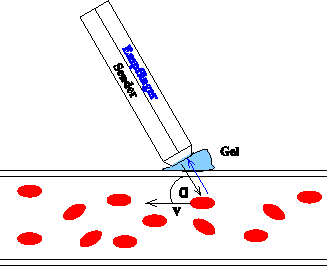
\includegraphics[width=\linewidth]{pictures/Skizze1.pdf}
    \caption{Die Doppler-Sonographie. \cite{us3}}
    \label{fig:Skizze1}
\end{wrapfigure}
Von Interesse ist der Doppler-Effekt auch in Anwendungen wie der Ultraschalltechnik, dargestellt in \hyperref[fig:Skizze1]{Abbildung (\ref{fig:Skizze1})}.
Da bewegte Objekte, wie beispielsweise Blutkörperchen, durch den Dopplereffekt in der Frequenz $\nu_0$ verschoben werden, liegt hier der Fall aus \hyperref[eq:doppler2]{Gleichung (\ref{eq:doppler2})} vor.
Durch den Winkel, denn der Beobachter/Empfänger einstellen kann, berechnet sich die Frequenzverschiebung über
\begin{equation}
    \increment \nu = \nu_0 \frac{v}{c}\left(\text{cos}(\alpha) + \text{cos}(\beta)\right).
\end{equation}
Da die beiden Winkel bei dem Impuls-Echo-Verfahren identisch sind, vereinfacht sich die Gleichung zu
\begin{equation} \label{eq:freqvers}
    \increment \nu = 2 \nu_0 \frac{v}{c} \text{cos}(\alpha).
\end{equation}

Die Erzeugung von Ultraschall ist über verschiedene Wege möglich.
Ein Weg ist die Anwendung des reziproken \textit{piezo-elektrischen Effektes}.
Dafür wird ein piezoelektrischer Kristall in ein elektrisches Wechselfeld gegeben, sodass dieser zu Schwingungen angeregt wird.
Bei Schwingungen strahlt dieser dann Ultraschallwellen ab.
Wird die Anregungsfrequenz so gewählt, dass die Eigenfrequenz des Kristalls getroffen wird, entsteht der Resonanzfall.
Dabei können große Amplituden und Schallenergiedichten erzeugt werden.
Der Kristall, meistens ein Quarz, kann auch als Empfänger genutzt werden.